% Version 2.20 of 2017/10/04
%
\documentclass{article}
%
\usepackage{graphicx}
% Used for displaying a sample figure. If possible, figure files should
% be included in EPS format.
%
% If you use the hyperref package, please uncomment the following line
% to display URLs in blue roman font according to Springer's eBook style:
% \renewcommand\UrlFont{\color{blue}\rmfamily}

\begin{document}
%
\title{Short Paper - Binding Bit Patterns To Boiler Tubes}
%
%\titlerunning{Abbreviated paper title}
% If the paper title is too long for the running head, you can set
% an abbreviated paper title here
%
%\author{Partha Das Chowdhury\inst{1}\and
%Bruce Christianson\inst{2}\and Hannan Xiao\inst{3}\and Sarajit Jha\inst{4}\and Dewal Narayan\inst{4}\and Kritee Ghosh\inst{1}\and Sanchari Chatterjee\inst{1}}
%
%\authorrunning{P.Das Chowdhury et al.}
% First names are abbreviated in the running head.
% If there are more than two authors, 'et al.' is used.
%
%\institute{VARA Technology  
%\email{\{partha.chowdhury,kritee.ghosh,sanchari.chatterjee\}@varatechnology.com}
% \and
%University of Hertfordshire
%\email{b.christianson@herts.ac.uk}  
%\and Kings College London \email{hannan.xiao@kcl.ac.uk} 
% \and Tata Steel \email{\{sarajit.jha,dewal\}@tatasteel.com}}
%
\maketitle              % typeset the header of the contribution
%
\begin{abstract}
Buyers and sellers enter into a compulsive trust relationship between each other, the reason being the buyer has no way to verify that a seller is trading in genuine products procured through proper channels. Such compulsive  trust relationships have serious safety implications. Manufacturers ship products with unique identifiers or markers or certificates on them as a mark of genuine produce and not counterfeit. We explore the conventional mechanisms to prevent counterfeits in safety critical boiler tubes. Our experience is that unique identifiers and certificates alone cannot prevent counterfeit. We advance the view that a combination of conventional identifying mechanisms and a participative (by the stakeholders) decentralised data layer will effectively bind bit patterns to real world entities.  To this end we implemented a blockchain platform for a large industrial partner to prevent counterfeits. Our work is significant in a world where safety and security are gradually merging. 

%\keywords{Counterfeit  \and Blockchain \and Steel tubes.}
\end{abstract}
%
%
%
\section{Problem Definition and Use Case}
Conventional efforts to ensure quality against counterfeit include printing identifiers on products, sometimes accompanied with certificates from the manufacturer. The identifiers~\cite{rja} include numbers, holograms, barcodes, radio frequency identification (RFID), IoT (Internet of Things) devices. Digital identifiers by themselves when used in isolation cannot address the problem of legitimate identities printed on counterfeit products~\cite{rja}. Bit patterns can be freely copied or modified, thus making any binding between a real world artefact and a bit pattern a difficult problem~\cite{binding}. %In this paper we present a implementation prevent the use of such identities on counterfeit products. %Thus, stopping at printing the unique identifier on a real world artefact will not eliminate the counterfeit problem. 

The contribution of this undertaking is, classical product identifiers used in combination with a decentralised programmable shared data layer, configures the affected parties into the system to participate to prevent counterfeits. 
%In this paper we propose, a combination of product identifiers and a participative decentralised shared data layer among all the stakeholders, to prevent counterfeit products with legitimate identifiers. 
We implemented our proposition for a real world safety critical product. Our system will ensure that in a supply chain network an entity which does not procure goods through legitimate channel will not be able to sell or propagate them in the supply chain network. We use boiler tubes for exposition however our system can be used for other products sold through a standard distributor/dealer network. 
%The manufacturer as well as the end customer participates to control the risks they are exposed to. The threat we address is selling a bad product with a legitimate identifier (issued by the Original Equipment Manufacturer). 
%\section{Use Case and Problem Definition}

A large steel manufacturer
%\footnote{{Acknowledgement}
%\begin{enumerate}
   %\item Professor Frank Stajano of University of Cambridge commented on the %earlier versions of this work and shared his ideas to address counterfeits %without certificate. We remain grateful to him for his kind suggestions.
%    \item This project was developed for Tata Steel Limited, one of the largest %steel manufacturers globally.
%\end{enumerate}},
manufactures boiler tubes. Boiler tubes are critical for safety. Boiler accidents lead to death,litigation and pay-outs by the manufacturer. Boiler tubes can only be sold with digitally signed (by the manufacturer) Test Certificate (TC) to guarantee that a particular boiler tube came from a particular manufacturer. 
%The test certificate 
A TC has all the physical characteristics of the particular tube with a one to one linking with the tube by a unique identifier (lot numbers) printed on both the tube and the TC. A boiler authority inspector which is a third party (statutory authority) would then inspect a tube along with the TC before a boiler is commissioned. 
%A tube is tied to the TC through the batch number and other identifiers explicitly mentioned in the TC and the tube.
By law boiler tubes cannot be sold or used without a TC issued and digitally signed by the manufacturer. Prior to the deployment of the system described in this paper, the manufacturer used to send digitally signed certificates (without the name of the end customer) to the distributor who would then pass them on (after endorsing them with the name of the buyer) to the buyer. So even if someone has a genuine tube (purchased from a black market) but because they are unable to produce the certificate for the tube, they cannot use it other than keeping it at home (which is realistically, unlikely and financially prohibitive for boiler tubes). In absence of the certificates the manufacturer has no liability either for accidents or casualties. So end user has no incentive to buy a tube without a certificate\footnote{When a low quality product is sold with a certificate and the good quality is either sold in the black market or kept at home is considered as separate threat.}.

%\section{The Uniqueness of Boiler Tubes}\label{unique}
 %The physical properties are an integral part of the test certificate. They are generated using the physical characteristic of the %individual tubes. However an inherent limitation is to enable the end customers to validate the same physical properties using the equipment only available with large manufacturers. The certificate (accompanying the tube) is the safety guarantee (as of now) so far as the quality\footnote{we discuss a different threat where a low quality product is sold with a certificate and the good quality is either sold in the black market or kept at home as a separate threat in section \ref{quality}} of the tube is concerned. So even if one purchases it in a black market (without a certificate) they will not be able to use it to set up a boiler. Setting up any boiler requires clearance from the Boiler Authority which is a statutory body. Boilers cannot be set up discretely with the community not being aware as any accident will not only affect the operator but also the community around. The Boiler inspectors will come and verify the TC against the tubes used to set-up the boiler. So even if someone has a genuine tube (purchased from a black market) and they are unable to produce the certificate for it, thus cannot use it other than keeping it at home (which is realistically unlikely). In absence of the certificates the manufacturer has no liability either for accidents and casualties. So end user has no incentive to buy a tube without a certificate. 
%\section{Case for Departure}
We found counterfeit tubes with the same digital identity printed on them as on a genuine digital certificate belonging to a genuine tube. A photocopy of the original certificate was being used for both the counterfeit and the genuine tube. %since the distributor had the signed certificates and became more powerful than either the manufacturer and the end customer). 
%There was no visibility across the system to prevent the co-existence of a fake and a genuine product with the same identifier. The manufacturer had no clue if the distributor was re-using a certificate. 
There was no way for a boiler inspector to distinguish between a genuine product and a fake product. Low quality fake tubes led to accidents (leading to deaths) making the manufacturer liable for damages and litigation. The ability to counterfeit stems from the inability to unforgeably tie a product identifier on the genuine TC to one and only one tube as well as one and only one customer.
%a product id (reflected in a TC) can be copied and used in a fake product. 
%Someone who does not procure (who doesn't possess a genuine product) from the legitimate channel can easily introduce a fake product into the distribution channel. Even an authorised distributor can sell both a tube procured through legitimate channel as well as counterfeit using the photocopy of a genuine TC. 
The process clearly gave both incentives~\cite{rosscrypto} and immunity 
%(due to the inability to participate by all the stakeholders) 
to deal in counterfeits.
%someone can sell both the real and the fake without being detected thus earning twice using the same certificate. Once a good left the manufacturer the entities in the sales channel became more powerful than the manufacturer and the end customer to induce counterfeits in the channel. The manufacturer only can control till the first point of sale which is its authorised distributors.The inability to prevent counterfeits has spawned a huge market where people sell counterfeits or products they have not procured through proper channel. This leads to financial loss to the manufacturer, loss of brand reputation as well as harming the end customer. 

\section{Motivation}
``Our experience in the banking industry tells us that the principal criterion of levels of fraud is not the back-end technology we use but how we validate that a transaction is valid or not as and when the said transaction happens"~\cite{rosscrypto}. Conventionally victims cannot participate to control the risks they are exposed to and the entities which can protect the victims do not have the incentives to do so~\cite{ross}. For our purposes one way was to enable the the customers to remotely access the SAP\footnote{Systems Applications and Products in Data Processing} of the manufacturer to request and validate each and every TC issued against the tubes manufactured information. However that will require frequent concurrent access to their database, which can be a security nightmare and a potential single point of failure/malice. %Moreover a distributed system still has the connotation of a central authority which manages the SAP; thus
Distributors or sellers are also not willing to having the manufacturer only as the sole repository and controller of all the transaction data. 
%An expanded SAP system does not balance the power equation rather shifts it from the distributor to the manufacturer. 

Upon a reasoned scrutiny of the alternatives the secure and practical option was creating a decentralised programmable shared (tamper proof) data layer where synchronisation happened in near real time (without delay) and each entity was not required to depend on a central authority (for finality). We proposed a closed implementation of the blockchain consensus~\cite{satoshi,wef2,wef3} between the manufacturer, distributor, dealer and customer, enabling a balanced power structure. Once the goods left the manufacturer the distributor or other entities in the channel does not get more powerful than the manufacturer to pass on counterfeits. Manufacturers as well as end customers can themselves participate to control the risks they are exposed to instead of depending on a remote third party (distributor/dealer) to protect them.   %The process of resolving conflicts (like say git) might not be optimum for our application; our goal was to check for frauds as and when transactions happen. 
%Every time a purchase (from the distributor and down below) would happen, 
%\begin{enumerate}
%\item
%The Blockchain platform will enforce the scarcity property. One cannot generate more TC corresponding to a particular batch than produced in the factory.This is done without any central authority and/or a intermediary. 
%\item
%For every TC generation the consent of the manufacturer, distributor/re-seller in the chain and acceptance by the customer is required. The end customer will explicitly request and accept a live TC from the system. The Blockchain layer will prevent any one entity to independently override the other; as can be the case in distributed systems.
%\item
%TC will be generated and digitally signed by the manufacturer. This will prevent replaying an old TC. 
%\item
%The manufacturer will have visibility till the last level of small customers who usually buy one or two boiler tubes. 
%\item
%Our consensus protocol is based on the byzantine generals problem; participation is based on permissions (permissioned nodes). We are not energy insensitive; by design enough participants do not have the incentive to defect to allow counterfeits. 
%\end{enumerate}
Our solution is based on the assumption that the end customer (at whose premises a boiler would be commissioned) has no incentive to knowingly accept a fake product.%thus will participate to protect himself from the risks he is exposed to (of counterfeits). 
\subsection{Related Work} We are not the first to propose the use of blockchain in supply chain in general and trace-ability in particular. Research in~\cite{Schmidt} makes a strong case for blockchain to address opportunistic behavior in supply chain while authors in~\cite{chen} proposed the use of blockchain for quality control. A team of experts from the industry and academia proposed a comprehensive toolkit~\cite{wef} for blockchain adoption in the supply chain. Food trace-ability has been proposed in~\cite{tian,walmart,jun} using of RFID, IoT. The steel industry too has seen prototypes~\cite{cao} combining blockchain and IoT. 
On the other hand considerable research has gone into addressing the limitations with RFID or NFC mechanisms. Mechanisms to prevent cloning of RFID tags was proposed in~\cite{lejla}, while authors in~\cite{nfc} propose mechanisms where a mobile phone can be used to verify a product offline.There are mechanisms which use the unique physical characteristics and their unique variations %is our next consideration. This will address to address threats to quality of products. 
One candidate is a physically unclonable function~\cite{pappu} to give a fingerprint. 
%which is included in the certificate. 
The goal is that it is so hard to modify a fake product to have the correct fingerprint, that it's enough to destroy the financial value proposition for the forger. %The second requirement is that genuine products are sufficiently robust to resist having their fingerprint changed by accident; the usual mechanical manipulations that products undergo during its supply chain travels. 

We prevent counterfeit without RFID and/or IoTs. A practical constraint is that not every customer is equipped with the required infrastructure to verify physically unclonable functions. Our implementation works with the existing product - identifier mapping. Our system does not discriminate against those who are digitally less matured and use feature phones. This was a requirement from our industrial partner as well. In trace-ability solutions~\cite{tian,walmart,jun} the end customer is mostly a passive verifier but do not participate to pre-empt counterfeits. 
%In our system a TC is not generated without the active consent of he customer to the blockchain layer. 
A scientific impact of our implementation is a customer actively participates to prevent counterfeits.   

\section{Technical Implementation}
\subsection{Our Goals}
%Our goal was to prevent use of unique digital identifiers on counterfeit products.
%The ability to re-use genuine certificates with low quality fakes took away the safety guarantee resulting in accidents at end customer premises and liability damages for the manufacturer.
Our goal was to ensure that genuine TCs are used with genuine tubes and not with low quality fakes; we ensured three properties for TC generation.
\begin{enumerate}
\item
Authenticity - For every TC generation the consent of the manufacturer, distributor/re-seller and acceptance by the customer is required. The end customer will explicitly request and accept a live TC from the system. The blockchain layer will prevent any one entity to independently override the other.
\item 
Liveness - TC generations will be live at the point of sale. 
%One cannot retrospectively issue a TC thus preventing any recycling of an old TC. 
Instead of sellers passing on the test certificate, the new process would have the end customer (who has no incentive to buy a boiler tube without a certificate) explicitly requests a certificate directly from the manufacturer, and receives it. 
\item 
Scarcity - %In our system %TC should be directly linked to the number of tubes manufactured. 
One should not not be able to produce or issue TC beyond the number of tubes manufactured for a particular lot. 
\end{enumerate}
All the entities including the customer will be able to independently validate that the identifier on the tube and TC exists only for one tube as well as one customer and not otherwise. 
%The shared layer %along with the identifying mechanisms wrests (power) control from the distributor and distributes power equally between the manufacturer, seller and the end customer.

\subsection{System Configuration}\label{configuration}
The types of entities are the manufacturer, the distributors, the dealers, end customers and the boiler authority (regulatory body). There is one manufacturer and one boiler authority but there are many distributors, dealers and end customers.  
%The end customer can be an organisation or a individual retail buyer. In case where the end customer is a organisation they become a node, for retail buyers they connect to the Blockchain platform via their mobile app. For retail buyers who have no access to internet and/or a smart phone we ensure the scarcity,liveness and authenticity property for them. 
\begin{figure}[ht]
\centering
  %  \includegraphics[width = 0.5in, natheight = 10, natwidth = 10]{architecture-diagram.png}
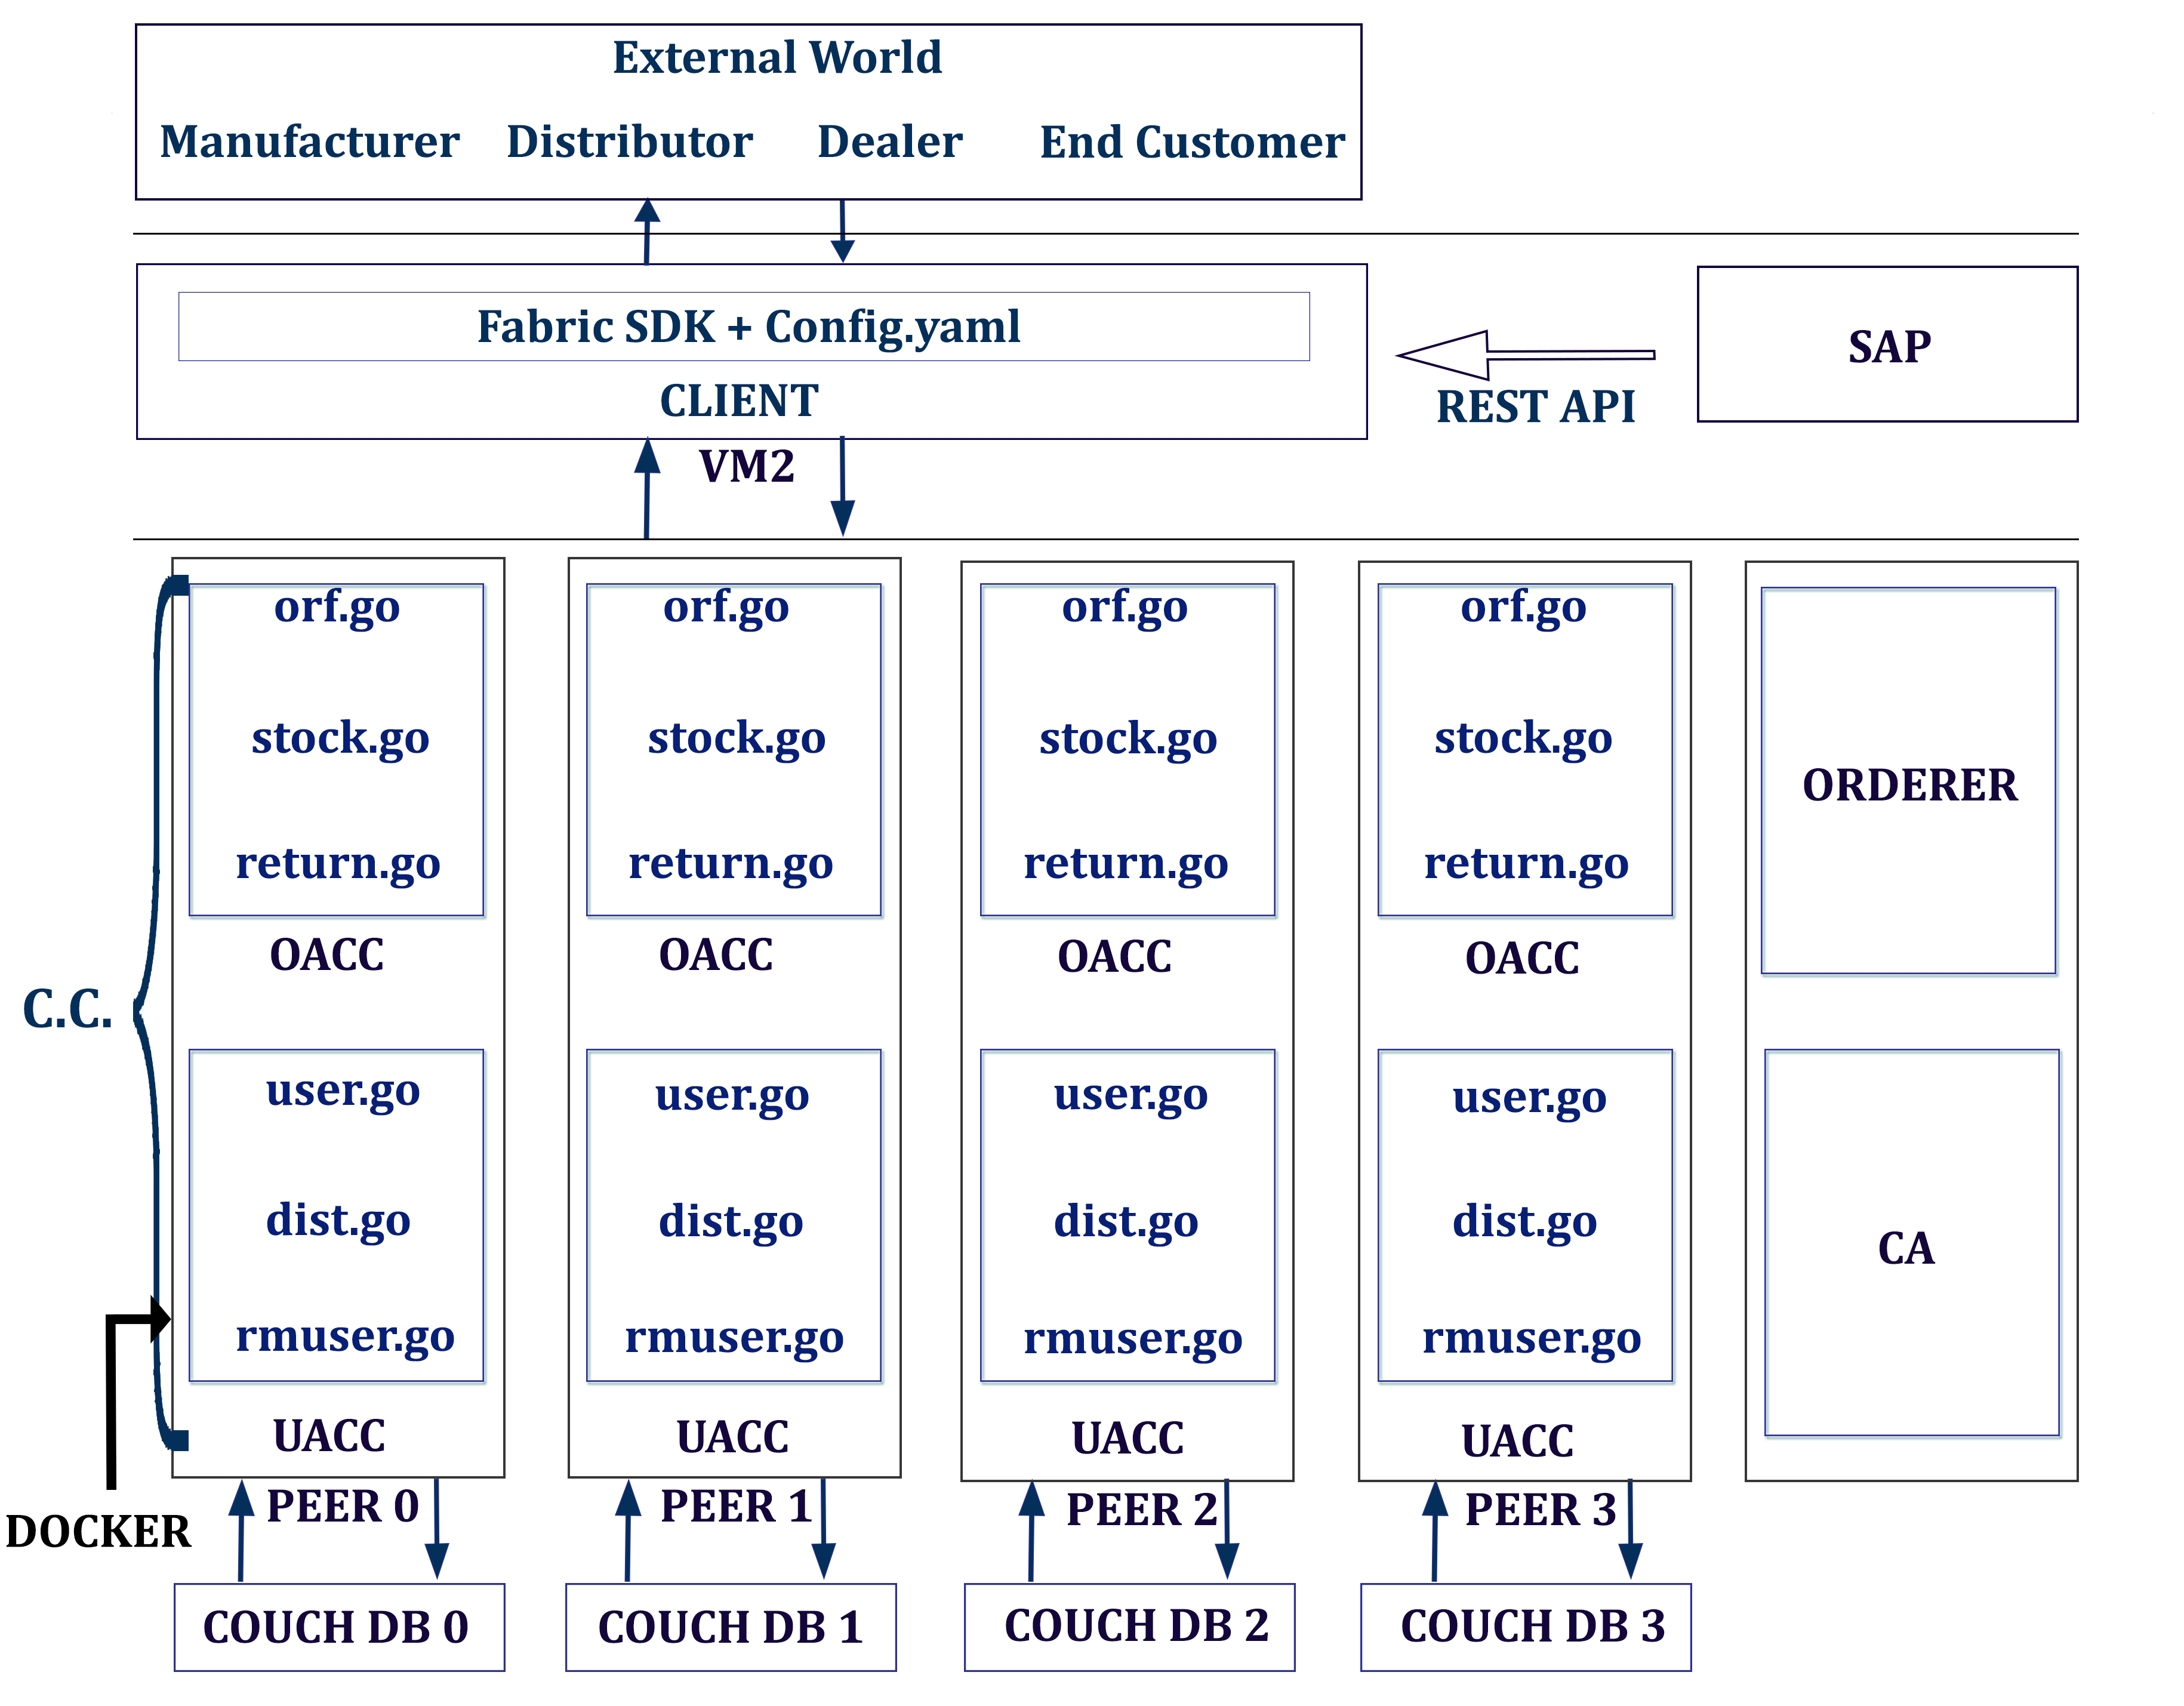
\includegraphics[scale=0.07]{Architecture-Diagram.png}
\caption{The Chain codes along with Orderer and CA}
\end{figure}
\begin{enumerate}
\item
The manufacturer, distributors, dealers' cloud has virtual machines (VM1 and VM2) as Figure 1. We have used VM1 to deploy our blockchain setup and VM2 is for web server setup (the Rest service). 
%VM1 of each entity does not connect with other entities while VM2 connects with the other entities. 
%\item
%VM1 has Hyperledger fabric, docker, docker images and Golang. VM2 has Golang, nodejs, Java,Python and fabric-sdk-go. The crypto-config file of VM1 is shared with VM2. The config.yaml file used in VM2 has details of the configurations of the peer. 
\item
%Each entity is defined as a role in the blockchain platform with associated permissions and their local database. 
The front end React native and web apps~\cite{react} connects (using HTTPs~\cite{tls} and JWT) each entity via the web server (VM1) to their back end Hyperledger smart contracts~\cite{hlf} (VM2) written in Golang. The OACC and UACC containers enforce the authenticity, liveness and scarcity properties. Each entity has their own local database.
% The container OACC enforces that no one (without legitimately procured tubes) in the channel can become a seller.
\item
Blockchain platform does not pull any data from the manufacturer's SAP. SAP always pushes data to the web server with an endpoint in a json format. The communication between web server and the SAP happens over a secure channel. 
\item
Every entity hosting the platform stores a hash of VM2 in VM1 inside the blockchain layer. 
%So in blockchain every peer stores the hash in its own ledger. 
Every transaction via the Rest Server carries the hash to the blockchain layer. If anyone makes any changes inside VM1 the hash will not match with the previously stored hash. If anyone wants to make any changes in VM2 inside the crypto-config file or in config.yaml file then the Rest server will not be able to connect the blockchain layer.
\item
There are three SOAP web services called by the web server. The services are provided by the manufacturer. One for digitally signing the TC. The second one is sending SMS to the Distributor and Dealer or End customer, finally one for terms and conditions.
%\item
%We have developed a Mobile Application and web application for connecting the user with the web server in React Js~\cite{react}. Mobile Application communicates with the web server with https request and every transaction carries a JWT. 
%\item
%Each peer independently validates every sell and issuance of TC from their respective state information. Then upon consensus state changes happen. The OACC and UACC containers enforce the authenticity, liveness and scarcity properties.The container OACC enforces that no one (without legitimately procured tubes) in the channel can become a seller.
\item
The boiler authority connects to the platform via a web interface and verifies (using the identifier) the proof of existence of a TC in the Blockchain layer. The platform confirms whether or not a
%; the Boiler authority via the portal ensures that 
certificate presented is a certificate issued by the manufacturer to a particular buyer for the identified tubes.
\end{enumerate} 

\subsection{The Revised Process Flow}
The revised process flow is shown in Figure 2.
%The most important user-facing change has been that TCs are issued at the point of retail sale further down the distributor, upon explicit request and consent of the buyer.  
\begin{figure}[ht]
\centering
 \includegraphics[scale=0.1]{to-be-tubes-updated.png}
\caption{A TC Issuing Process}
\end{figure}
\begin{enumerate} 
\item
Every purchase (by a distributor from the manufacturer) is committed to the SAP. However no certificates are issued to the distributor at this stage. 
\item
SAP pushes the purchase details along with the required fields for TC to the blockchain layer.  
\item
A dealer/end customer initiates a purchase from a distributor. 
\item
The distributor completes the sale process through the blockchain platform using the mobile app or the web app. 
\item
The platform initiates a challenge-response with the buyer through a (OTP) for liveness and authenticity. The buyer explicitly confirms the purchase to the platform.
\item
Once the buyer explicitly requests a TC to the blockchain platform after a purchase signed certificates are sent to the buyer email id. 
%The same process is repeated for smaller re-sellers who buy from the dealer as well as when they sell to the fabricators. TCs are no longer being issued along with the consignments.
\item
Boiler inspector logs into the portal to verify that the certificate presented is indeed a certificate issued by the manufacturer to the particular buyer for the identified tubes.  
\end{enumerate}
%With our solution one cannot request certificates (unless they legitimately own the tubes and bought them in proper channel) thus any tube without a certificate is of no use (apart from keeping them at home). 
%The threat we addressed was selling a bad tube with a good certificate which makes the manufacturer liable and result in casualty for the end customer.

\subsection{System Adaption}
Our goal was that users in a distributor dealer based network can adapt our system with minimal disruption and marginal cost. 
\begin{enumerate}
\item
For the manufacturer, distributor, dealers and B2B customers we publish an end point to connect their SAP to the Blockchain. 
%\item
The cloud blockchain configuration is at the back end and invisible to the users of the respective organisations. The mobile app and web version is designed to align with their existing usability experiences.
%For the manufacturer they keep working with their SAP as they used to while for others they keep working on a web/mobile interface as they used to earlier.We organised a training and ensured that no more than extra two steps are required to complete a order and request a TC. 
\item
For customers without a smart phone or internet we do not need them to install any software or use a web application. We assume they have a feature phone which receives a OTP. Every time a purchase is made by a retail customer an OTP is sent to them to ensure the liveness property. The customers are made aware through massive publicity campaigns. 
\end{enumerate}

\subsection{Performance Testing}
The old process was manual (distributors printed TCs for customers). We test\footnote{https://jmeter.apache.org/} response times for our system (figure 3). 
Accept return and initiate return (involved a OTP being sent over mobile networks) took 4.3 and 4.5 seconds respectively. The elapsed time for a buy confirmation is .73 seconds. The average response time for TC generation is 134 ms. From the total distributor population of 123 we sent 100 simultaneous requests where each seller had a backlog of 2000 pending orders. Usually the maximum pending order of a seller is not above 50. We experienced 5.4 seconds for dashboard while 10.4 s for order history and .99 seconds for each order detail. The throughput for order history with extraordinary backlog is 211 kb/sec.
%The total number of distributors, dealers and small retailers is between 100-130 spread across the country. 
%The year on year sale range between 1,00,000 metric ton (MT) to 1,30,000 MT.
% The old process was manual (distributors printed TCs for customer). The users wanted to know the response times for transactions using our application. The test\footnote{https://jmeter.apache.org/} result is as (figure 3). 
 %We are also aiming a 2\% increase in annual sales in FY2020-2021 as a direct benefit of this platform.
\begin{figure}[ht]
\centering
  %  \includegraphics[width = 0.5in, natheight = 10, natwidth = 10]{architecture-diagram.png}
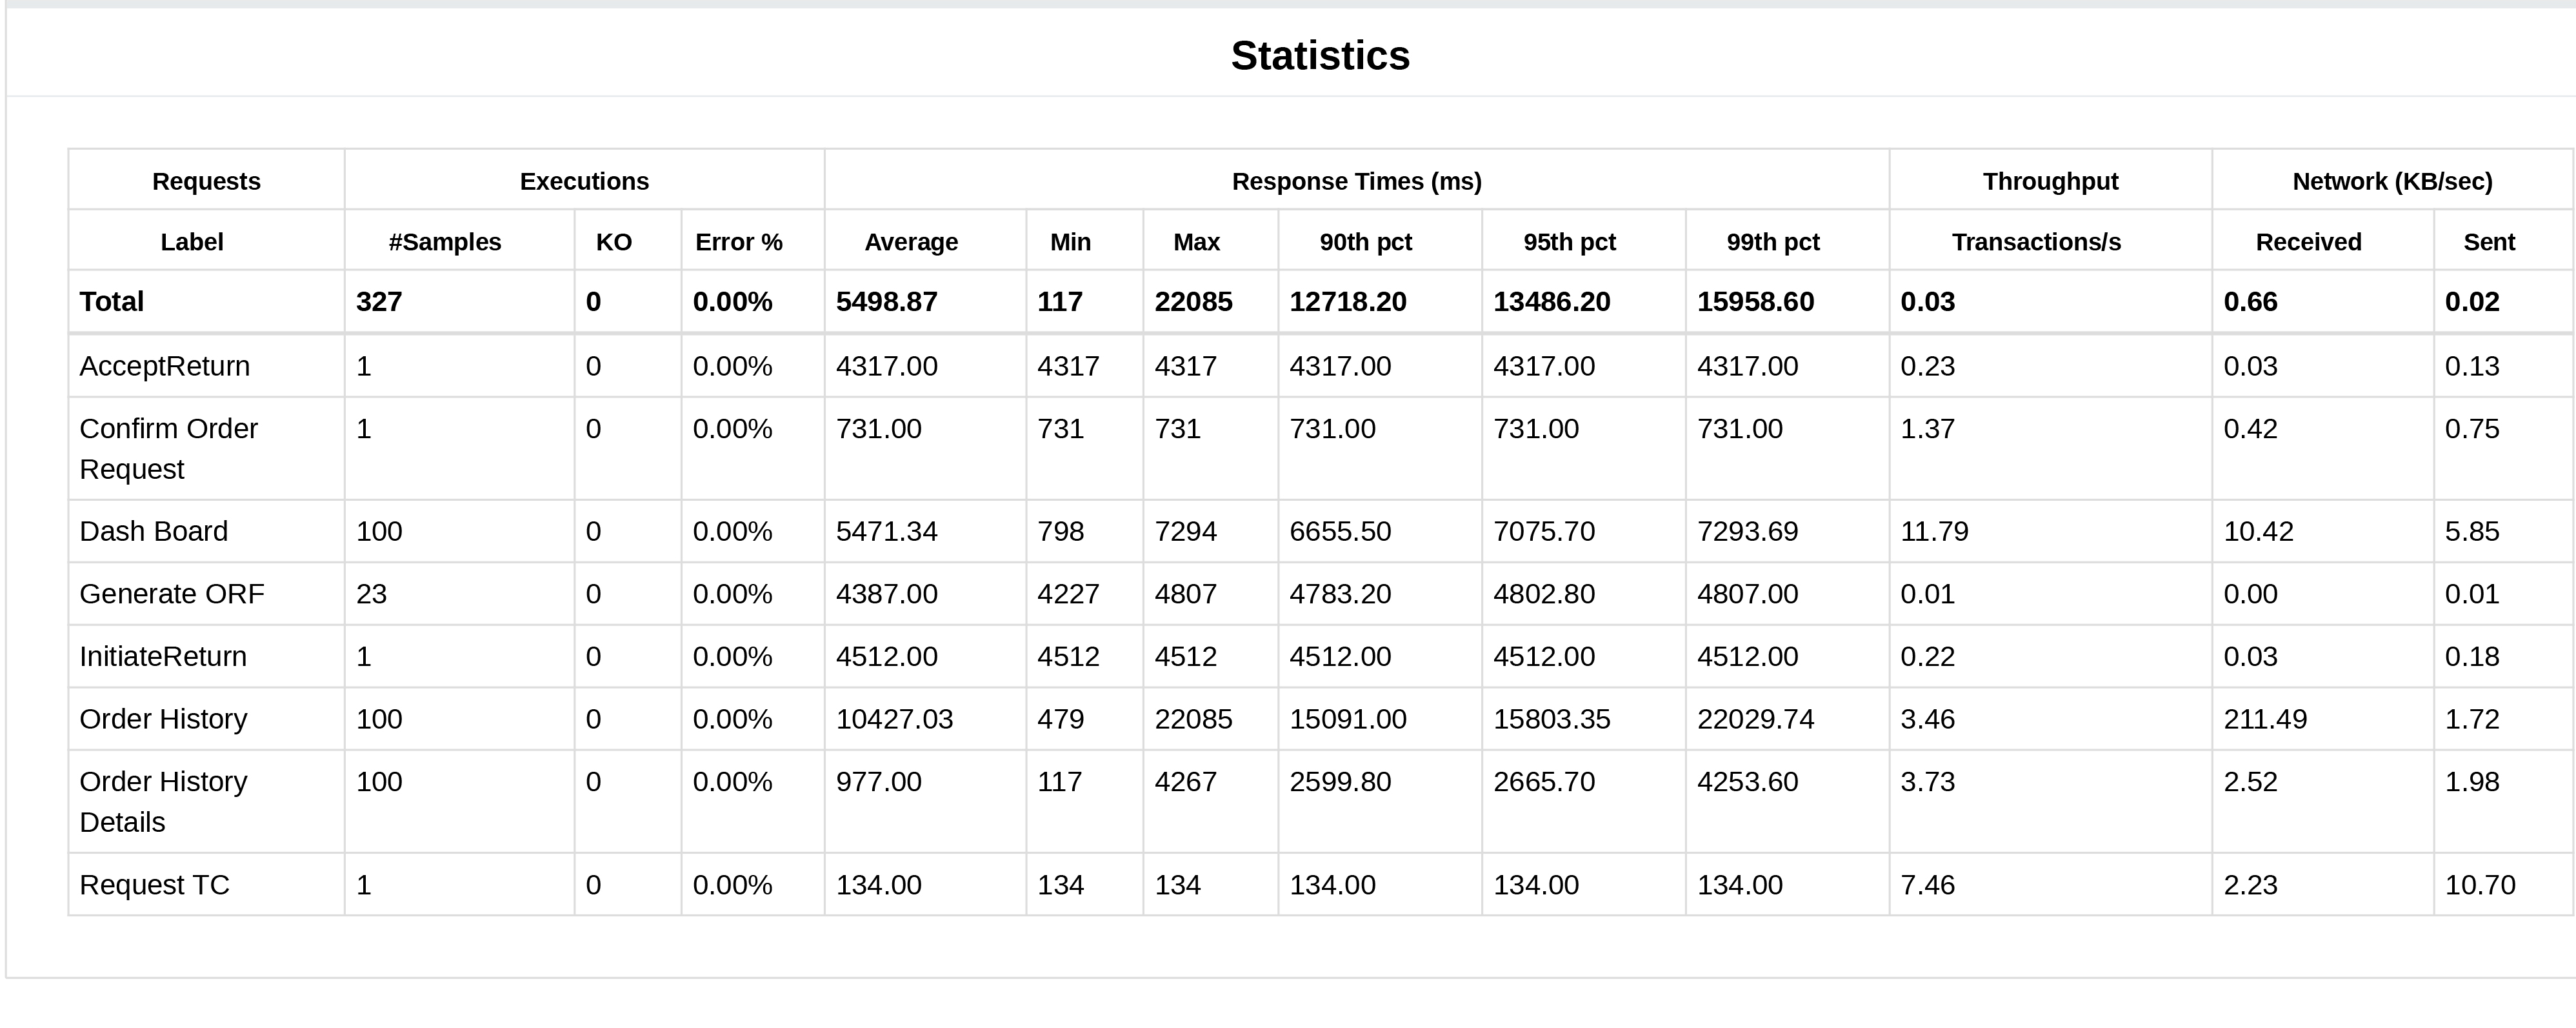
\includegraphics[scale=0.20]{DealerR.png}
%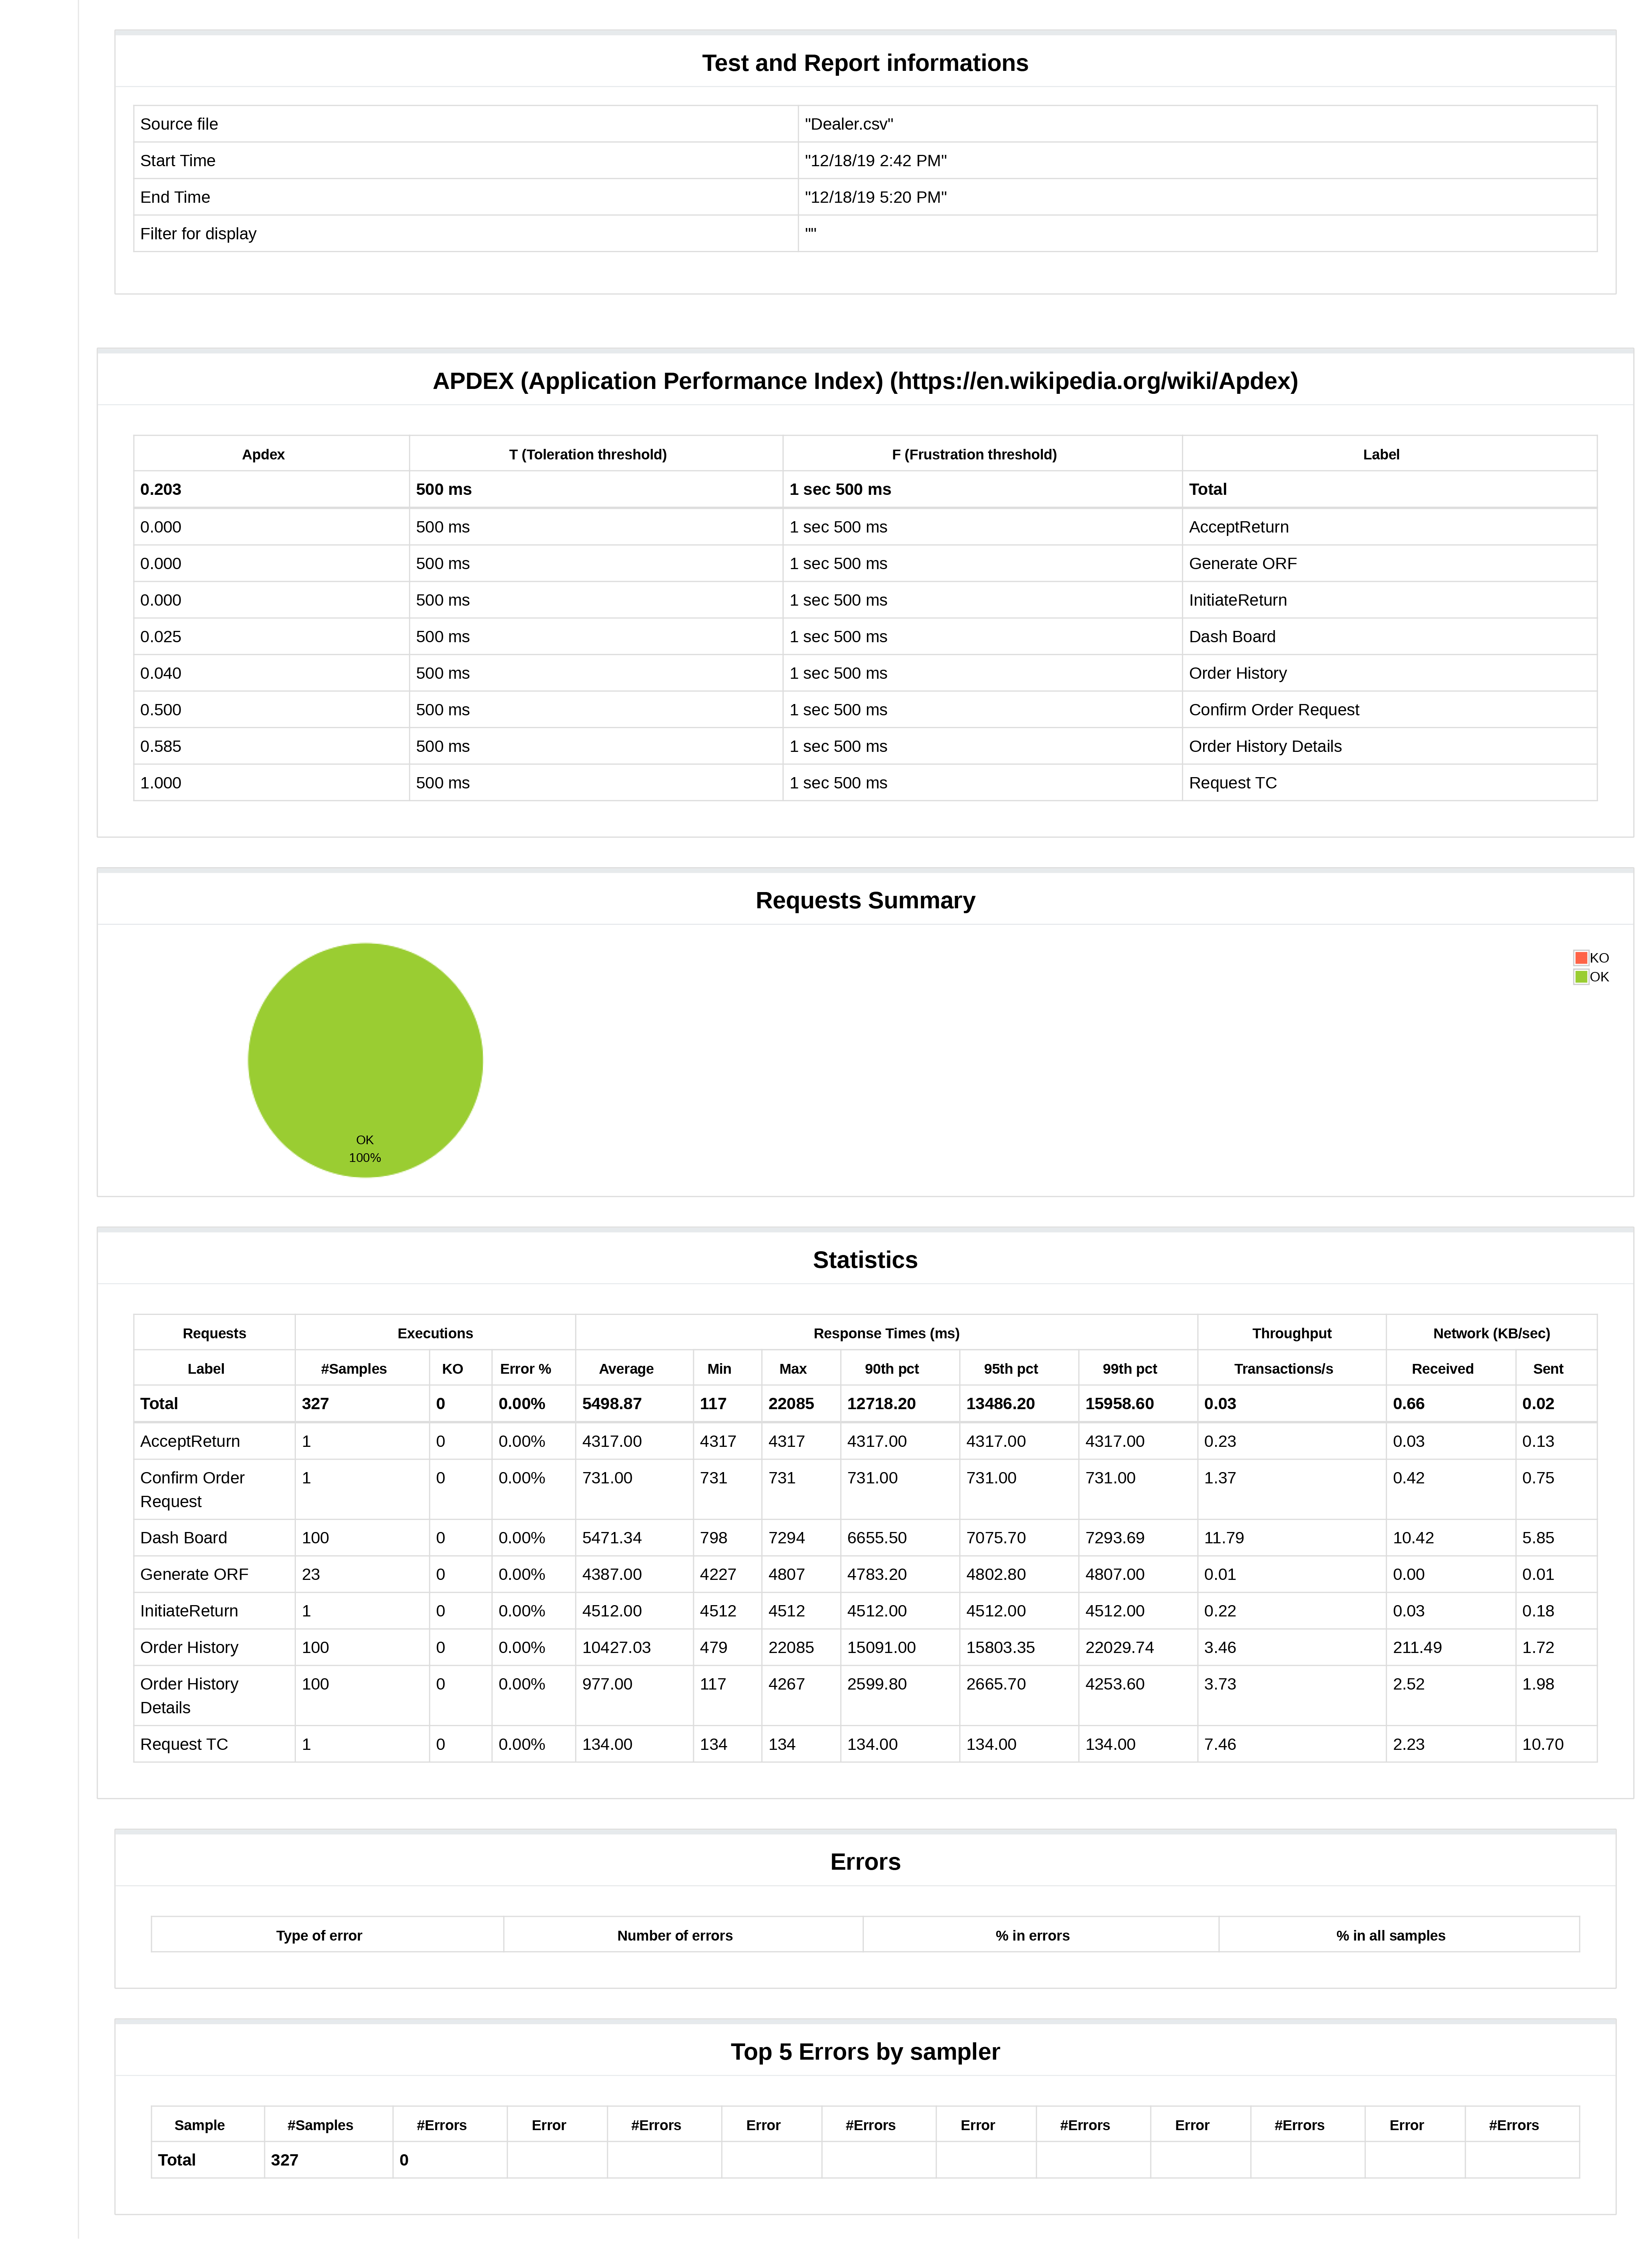
\includegraphics[scale=0.09]{Dealer.png}
%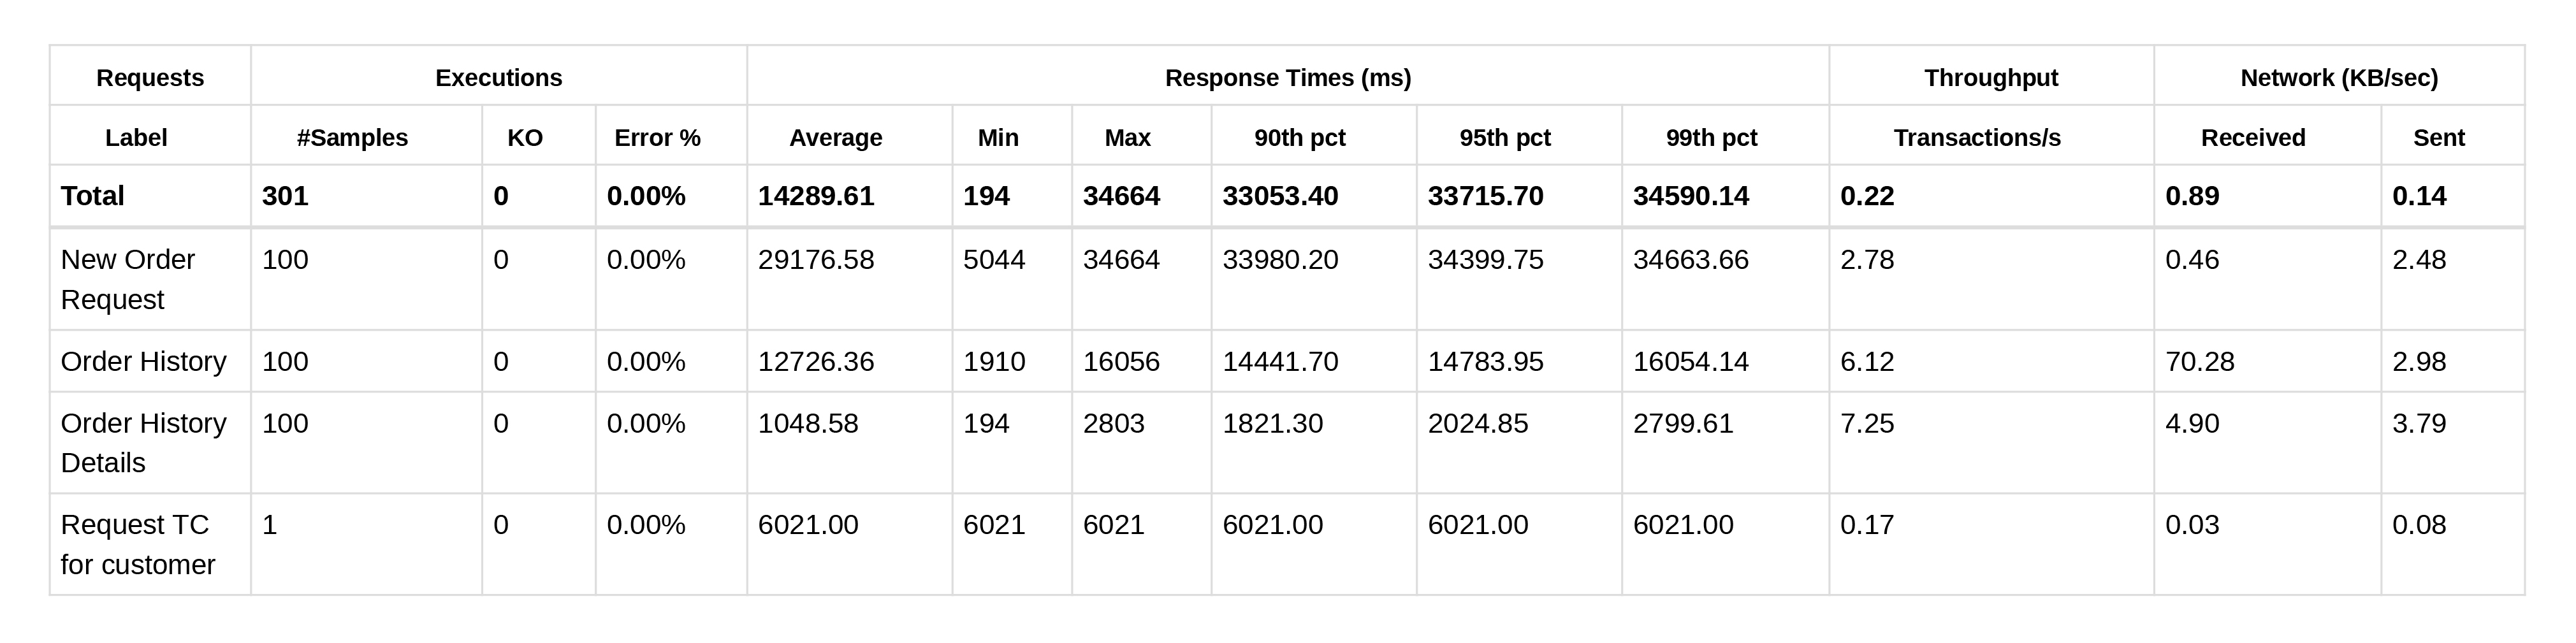
\includegraphics[scale=0.09]{ManufactureR.png}
\caption{Response Time}
\end{figure}

\section{Future Directions- Nemo Dat Quad Non Habet}\label{quality}
Our goal was to prevent the ability to re-use certificates by malicious middlemen; we took the power away from the distributor, configured the manufacturer and the end customer. Any entity which does not or cannot legitimately possess a genuine good will not be able to pass it on further down the line. Our solution would address the threats to counterfeit in supply chain scenarios where a customer is participating to seek authenticity of the goods. Traditionally there has not been much success in configuring the affected parties (in case of malice and/or incompetence) into the system~\cite{ross}. We configure the affected parties who suffers the most in case of counterfeit into the system~\cite{pdc2010}. 

%There are products which can be kept at home unlike boiler tubes or someone is happy to buy in the black market without the certificate. Our system to be widely applicable would need to work with such products as well. 
For many products other than boiler tubes, a crooked operator in the supply chain can substitute a genuine product of good quality for one of poor quality, passing on the latter with the certificate for the good one. (OK, they can’t resell the good one with a certificate, but they can install it in their own luxury home.) 
%Or sell it to someone who’s happy to get it at a reduced price without a certificate on the black market, because they can see it’s good quality anyway.) 
%The manufacturer also manufactures tubes for the automotive industry, tubes used for multi storey structures which can be put to other uses (including domestic use). 
%Working with the unique physical characteristics and their unique variations is our next consideration. This will address threats to quality for products. A reasonable way to ensure the integrity of the natural variation (of a product) information is to use a physically unclonable function~\cite{pappu} (of the physical properties) to give a fingerprint, which is included in the certificate. The goal is that it is too hard to modify a fake product to have the correct fingerprint, it's enough to destroy the financial value proposition for the forger. The second requirement is that genuine products are sufficiently robust to resist having their fingerprint changed by accident; the usual mechanical manipulations that products undergo during its supply chain travels. 
%including being picked up by forklift trucks, being taped to other pipes, being bumped around. Perhaps sampling a suitable location on the inside of the pipe might be valuable, as better protected from injury. 
A realistic way would be to enable the end customer to be able to validate such products against the results of the physically unclonable function in the certificate. Even if multiple tubes are exact clones\footnote{However, exact clones destroy the financial value of the forger.} of each other 
%(with the assumption that they will produce similar fingerprints) 
the Blockchain platform can complement by enforcing the scarcity property, the authenticity and liveness property for the end customer (indemnifying the manufacturer from litigations). 

%\section{Nemo Dat Quod Non Habet}
%We proposed to address this particular problem by enforcing that any entity which does not or cannot legitimately possess a genuine good will not be able to pass it on further down the line. Our solution would address the threats to counterfeit in supply chain scenarios where a customer is participating to seek authenticity of the goods bought directly from the manufacturer. Blockchain based consensus mechanisms facilitate such enforcement mechanisms by bringing all the stakeholders into one platform. Moreover the user and the manufacturer are the two most affected entities in case of low quality counterfeits; traditionally there has not been much success in configuring the affected parties (in case of malice and/or incompetence) into the system~\cite{ross}. Blockchain configures the affected parties into the system in a manner that the entity which suffers the loss in case of counterfeit is configured in the system~\cite{pdc2010}. 
%In the old process the distributor became more powerful than the manufacturer and the end customer; however now the various entities are equally powerful in the way that a distributor will not be able to remain insulated from the manufacturer and insert counterfeits (as could have been done before). Digital identifiers such as barcodes etc. used in isolation without blockchain cannot guarantee that all of them will participate in all the transactions at every step of the process. The visibility and oversight of the manufacturer will prevent someone (without a legitimate product) to introduce counterfeits in the system. If a holder of a genuine product tries to introduce counterfeit then he can do it only to his peril; he can either sell the counterfeit or the genuine product but not both; thus there is a financial dis-incentive for him to deal in counterfeits. 





% ---- Bibliography ----
%
% BibTeX users should specify bibliography style 'splncs04'.
% References will then be sorted and formatted in the correct style.
%
\bibliographystyle{plain}
\bibliography{dissertation}
%


\end{document}
